\documentclass[11pt,letterpaper]{article}
\pdfinfoomitdate=1\pdftrailerid{}\pdfsuppressptexinfo=15
\usepackage[T1]{fontenc}\usepackage[utf8]{inputenc}
\usepackage{lmodern,mathpazo,microtype}
\usepackage[margin=.88in,headheight=15pt]{geometry}
\usepackage{amsmath,amssymb,amsthm,mathtools}
\usepackage{graphicx,xcolor,booktabs,tabularx,array,enumitem,tikz}
\usetikzlibrary{arrows.meta,positioning,calc,fit,backgrounds}
\usepackage{titlesec,fancyhdr,needspace,placeins,listings,xurl}
\usepackage[numbers,sort&compress]{natbib}
\definecolor{ink}{HTML}{151224}\definecolor{violet}{HTML}{6842A2}
\definecolor{gold}{HTML}{B18740}\definecolor{mint}{HTML}{176E68}
\definecolor{brightgold}{HTML}{EDC277}\definecolor{brightmint}{HTML}{A0E1D2}
\definecolor{pale}{HTML}{F2EFF7}\definecolor{muted}{HTML}{61596E}
\usepackage[colorlinks=true,linkcolor=violet,citecolor=violet,urlcolor=mint,bookmarksnumbered]{hyperref}
\hypersetup{pdftitle={FLYWHEEL OMEGA: The Economy as an Output},pdfauthor={Vincent Boucher},pdfsubject={Transformational Intelligence for constructing economically viable games and their successors},pdfkeywords={FLYWHEEL OMEGA, Transformational Intelligence, mechanism design, economic possibility, constructive succession, strategic composition}}
\urlstyle{same}\setlength{\emergencystretch}{3em}
\widowpenalty=10000\clubpenalty=10000\displaywidowpenalty=10000
\setlength{\parindent}{0pt}\setlength{\parskip}{5pt}\linespread{1.025}
\newcolumntype{Y}{>{\raggedright\arraybackslash}X}
\newcolumntype{P}[1]{>{\raggedright\arraybackslash}p{#1}}
\newcommand{\repo}{https://github.com/MontrealAI/AGI-Alpha-Invention-Flywheel-Lab}
\newcommand{\omegaFW}{FLYWHEEL~$\Omega$}
\newcommand{\lead}[1]{\Needspace{5\baselineskip}\par\medskip\noindent{\large\sffamily\bfseries\color{violet}#1}\par\smallskip}
\newcommand{\thesis}[1]{\par\medskip{\sffamily\bfseries\large\color{violet}#1}\par\medskip}
\newtheorem{proposition}{Proposition}\newtheorem{definition}{Definition}
\newtheorem{corollary}{Corollary}
\setlist{leftmargin=1.35em,itemsep=3pt,topsep=5pt}
\renewcommand{\arraystretch}{1.18}\setlength{\tabcolsep}{5pt}
\titleformat{\section}{\Large\sffamily\bfseries\color{ink}}{\color{violet}\thesection}{.6em}{}
\titleformat{\subsection}{\normalsize\sffamily\bfseries\color{ink}}{\thesubsection}{.6em}{}
\titlespacing*{\section}{0pt}{18pt}{8pt}\titlespacing*{\subsection}{0pt}{12pt}{5pt}
\pagestyle{fancy}\fancyhf{}\fancyhead[L]{\footnotesize\sffamily FLYWHEEL $\Omega$}
\fancyhead[R]{\footnotesize\sffamily THE ECONOMY AS AN OUTPUT}
\fancyfoot[L]{\scriptsize\sffamily MONTREAL.AI / QUEBEC.AI}\fancyfoot[R]{\small\color{violet}\thepage}
\renewcommand{\headrulewidth}{.3pt}
\lstset{basicstyle=\footnotesize\ttfamily,columns=fullflexible,breaklines=true,keepspaces=true,showstringspaces=false}
\renewcommand{\topfraction}{.95}\renewcommand{\bottomfraction}{.9}\renewcommand{\textfraction}{.05}\renewcommand{\floatpagefraction}{.8}
\begin{document}
\hypersetup{pageanchor=false}
\begin{titlepage}\pagecolor{ink}\color{white}\thispagestyle{empty}

\begin{tikzpicture}[remember picture,overlay]
\fill[violet!30!ink] ([xshift=1.5cm,yshift=-6cm]current page.north east) circle (7cm);
\foreach \r in {4.2,5.0,5.8,6.6}{\draw[white,opacity=.045,line width=.7pt] ([xshift=1.5cm,yshift=-6cm]current page.north east) circle (\r cm);}
\draw[brightgold,line width=1.3pt] ([xshift=2.2cm,yshift=2.5cm]current page.south west)--([xshift=19.4cm,yshift=2.5cm]current page.south west);
\end{tikzpicture}
{\sffamily\small MONTREAL.AI / QUEBEC.AI\hfill\color{brightgold}RESEARCH EDITION 1.0}\par
\vspace{20mm}
{\sffamily\bfseries\fontsize{48}{54}\selectfont FLYWHEEL $\boldsymbol{\Omega}$}\par
\vspace{11mm}
{\sffamily\bfseries\fontsize{32}{37}\selectfont THE ECONOMY\\[6pt]AS AN OUTPUT}\par
\vspace{9mm}
{\sffamily\color{brightmint}\large TRANSFORMATIONAL INTELLIGENCE $\boldsymbol{\infty}$}\par
\vspace{5mm}
{\large Constructing better economic games\\and the means of their successors}\par
\vspace{10mm}
\begin{center}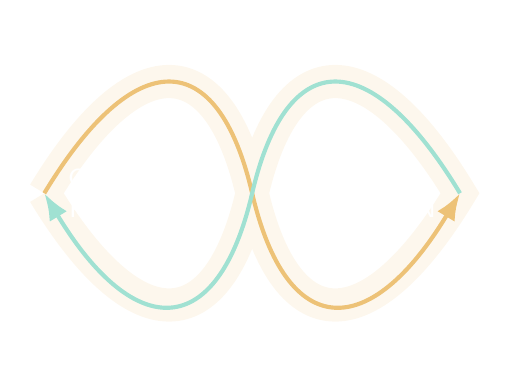
\begin{tikzpicture}[>=Latex,scale=.88]
\draw[brightgold,opacity=.13,line width=12pt] (-3,0) .. controls (-1.7,2.15) and (-.5,2.15) .. (0,0) .. controls (.5,-2.15) and (1.7,-2.15) .. (3,0) .. controls (1.7,2.15) and (.5,2.15) .. (0,0) .. controls (-.5,-2.15) and (-1.7,-2.15) .. (-3,0);
\draw[brightgold,line width=1.5pt,->] (-3,0) .. controls (-1.7,2.15) and (-.5,2.15) .. (0,0) .. controls (.5,-2.15) and (1.7,-2.15) .. (3,0);
\draw[brightmint,line width=1.5pt,->] (3,0) .. controls (1.7,2.15) and (.5,2.15) .. (0,0) .. controls (-.5,-2.15) and (-1.7,-2.15) .. (-3,0);
\node[text=white,font=\sffamily\small,align=center] at (-1.55,0) {CONSTRUCT\\POSSIBILITY};
\node[text=white,font=\sffamily\small,align=center] at (1.55,0) {ENABLE\\SUCCESSION};
\end{tikzpicture}\end{center}
\vfill
{\sffamily\bfseries\large The next breakthrough may be the game\\that makes it possible.}\par\vspace{8mm}
{\large\bfseries Vincent Boucher}\par\smallskip
President of MONTREAL.AI\par
MONTREAL.AI\quad\textbullet\quad QUEBEC.AI\par\medskip
{\small\color{white!75}Montr\'eal, Qu\'ebec, Canada\quad\textbullet\quad 3 November 2026}
\vspace*{13mm}
\end{titlepage}\nopagecolor\color{ink}\hypersetup{pageanchor=true}

\thesis{Intelligence can make cooperation itself a productive invention.}
\begin{abstract}
An intelligent enterprise can search for a better move within a supplied economic game. A more consequential enterprise can construct the production methods, evidence, interfaces and voluntary commitments that make a better game possible. We develop this second objective as \emph{the economy as an output}: an executable productive arrangement whose participants can achieve worthwhile outcomes together, whose complete costs and obligations can be funded, and whose retained capabilities can enable further arrangements. The paper extends the Transformational Intelligence and SUPER ALPHA research program by making the connection between productive capability and strategic possibility explicit. A new instrument changes what can be delivered; it can also change what buyers, suppliers and rivals can do. We formalize this connection, derive an exact effective tariff for composed offers, and provide a reproducible authored construction study. In its positive witness, a connector and verified staging together require five opening units, versus seven for staging alone and nine for final payment, at the same total process cost of nine. An equally permitted conventional constructor finds the same joint arrangement; with more capital, a conventional pure bundle earns more. An independently replayed public mechanism supplies a complementary warning: all 72 modeled single-report incentive checks pass, yet two component purchases obtain the joint services for 213 cents less. We connect actual choices and collections to timed finance, capability inheritance and separate tests of improved invention. The result is a constructive research program with exact analytical results and source-bound engineering evidence. Its ambition is a machine that repeatedly makes valuable cooperation possible and uses what succeeds to construct more consequential successors.
\end{abstract}

\textbf{The central question.} What valuable activity could become possible if intelligence could continually discover and construct the missing means of mutually beneficial cooperation?

\textbf{The thesis.} A complete economic invention includes what participants can produce, what they can verify, what they can choose, what they can commit, and what the arrangement leaves them able to do next. The game and its productive means must be constructed and tested together.

\textbf{The new step.} Earlier papers connect purpose-preserving reformulation, productive capability, viable exchange and funded succession. Here, the productive construction also determines the relevant strategic action space. We connect a concrete omitted-action failure to a constructive correction, an exact finite study, and an evaluation design that distinguishes a better arrangement from a better inventor.

\textbf{Evidence scope.} The new companion is an authored, exhaustive analytical study. The repository case is a pinned, independently replayed semantic counterexample plus a source review of historical simulations. Those simulations, their original capital and their failures remain separate. No actual customer revenue, physical deployment or US\$3 billion trailing-year profit is reported.

\clearpage
\section*{A reader's map}
\addcontentsline{toc}{section}{A reader's map}
\begin{tabularx}{\linewidth}{@{}P{3.1cm}YP{2.1cm}@{}}\toprule
Question & The answer developed here & Read\\\midrule
What is being invented? & A complete productive arrangement, including the conditions of useful voluntary cooperation. & Sections~\ref{sec:construction}--\ref{sec:related}\\
What can make a correct model fail? & Participants can compose the very capabilities that the model treats as separate choices. & Section~\ref{sec:strategic}\\
Can the obstruction lead to construction? & An exact finite study searches production and offers jointly, with complete composed choices and strong alternatives. & Section~\ref{sec:study}\\
What makes it a flywheel? & Executed delivery, available funds, inherited means and fresh successor acceptance are causally connected. & Section~\ref{sec:succession}\\
Has the inventor improved? & A separate comparison holds available content and equipment fixed while varying the invention procedure. & Section~\ref{sec:inventor}\\
What is established today? & Finite engineering capabilities, exact models, preserved conventional ties and a consequential model-boundary finding. & Section~\ref{sec:evidence}\\
What could follow? & Scientific, industrial and organizational arrangements that make important new work economically reachable. & Section~\ref{sec:horizon}\\\bottomrule
\end{tabularx}

\vspace{6mm}
\begin{figure}[h!]
\centering
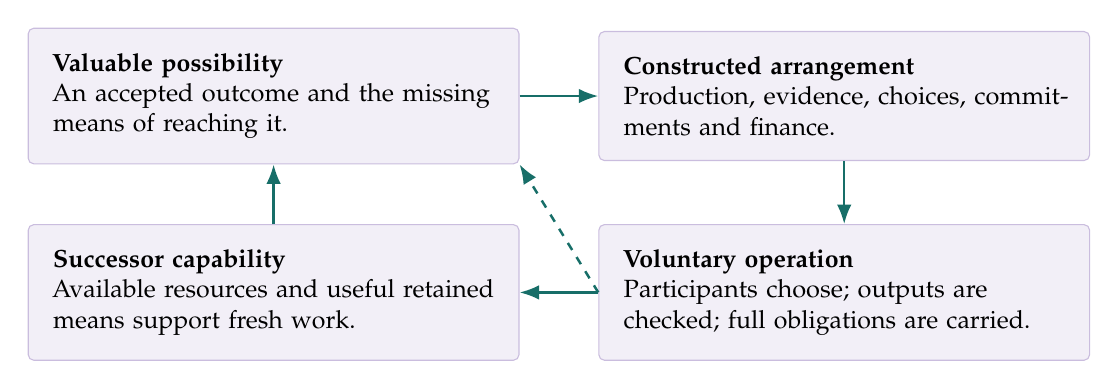
\begin{tikzpicture}[>=Latex,node distance=8mm and 10mm,
 box/.style={draw=violet!35,rounded corners=2pt,fill=pale,text width=5.6cm,minimum height=1.35cm,align=left,font=\small,inner sep=9pt},
 arr/.style={->,line width=.9pt,draw=mint}]
\node[box] (purpose) {\textbf{Valuable possibility}\\An accepted outcome and the missing means of reaching it.};
\node[box,right=of purpose] (game) {\textbf{Constructed arrangement}\\Production, evidence, choices, commitments and finance.};
\node[box,below=of game] (delivery) {\textbf{Voluntary operation}\\Participants choose; outputs are checked; full obligations are carried.};
\node[box,left=of delivery] (successor) {\textbf{Successor capability}\\Available resources and useful retained means support fresh work.};
\draw[arr] (purpose)--(game);
\draw[arr] (game)--(delivery);
\draw[arr] (delivery)--(successor);
\draw[arr] (successor)--(purpose);
\draw[arr,dashed] (delivery.west) -- (purpose.south east);
\end{tikzpicture}
\caption{The proposed loop. Each arrow requires evidence in a particular execution. The dashed return carries counterexamples into a revised construction. A profitable transaction, reusable capability and improved invention procedure remain distinct achievements.}
\label{fig:loop}
\end{figure}

\textbf{Research continuity.} \emph{Transformational Intelligence: Learning to Change the Game} remains the flagship conceptual reference, and \emph{AGI ALPHA: A Scalable Substrate for Intelligence Organizations} the foundation. This additive manuscript preserves their original results and scope \cite{ti,foundation}.
\clearpage

\section{Make valuable cooperation possible}\label{sec:construction}
Some opportunities cannot be captured by performing an existing job more cheaply. The valuable job is not yet a viable activity. Its output may be difficult to measure, its production method unavailable, its fixed cost too large for one participant, its commitments impossible to coordinate, or its risks difficult to assign. An optimizer inside the inherited arrangement can improve many decisions while leaving the decisive obstacle intact.

A different question begins earlier: what would have to exist for the activity to become worthwhile? A measurement can make a promise checkable. A shared instrument can make several separate investigations affordable. A qualified interface can allow otherwise incompatible capabilities to work together. A staged commitment can make a construction financeable without pretending that a promised payment is available cash. These are possible objects of invention, alongside algorithms and physical devices.

\emph{The economy as an output} names this constructive object at the scale of a particular arrangement or connected family of arrangements. It does not mean that one machine designs an entire society, fixes everyone's preferences, or obtains authority over independent participants. The output is a proposal that can be built, tested, voluntarily accepted, operated and improved. It includes a legitimate way to decline.

The distinction matters to the ambition of \omegaFW. The enterprise should discover outcomes worth creating, construct their missing means, and find terms under which the necessary participants prefer involvement to available alternatives. The resulting surplus can sustain the producer, while useful instruments and earned resources support further construction. A successful first arrangement can become an input to another.

\subsection{Preserve the purpose while changing the means}
Transformational Intelligence separates the authorized purpose from inherited problem formulations, intermediate goals and evaluation instruments \cite{ti,original}. A buyer may need a dependable maintenance decision, while an inherited workflow demands reconstruction of every hidden physical variable. Better sensing is one possible answer. A different decision procedure that needs only a sufficient observation is another. Either must still meet the maintenance purpose and its consequences.

Economic construction requires the same discipline. Replacing a difficult acceptance test with an easy but irrelevant proxy does not create the required outcome. Calling a deposit revenue does not finance a loss. Removing an inconvenient outside option from a model does not make participation voluntary. Conversely, a costly prerequisite of one delivery method need not remain a prerequisite of the beneficiary's actual purpose.

We therefore keep three things separate: the authorized outcome, constraints that genuinely bind the work, and choices inherited from the current implementation. During opportunity discovery, a different useful outcome may be proposed openly. During a comparison, the required purpose, rights, quality, risk and deadlines are fixed. The means remain available for invention.

\subsection{The complete arrangement}
Represent a proposed arrangement by
\begin{equation}
g=(y,m,v,N,A,I,T,f,\pi),
\end{equation}
where $y$ is the beneficiary outcome, $m$ the productive means, $v$ the evidence and acceptance method, $N$ the participants, $A$ their feasible actions, $I$ their information, $T$ the transfers and obligations, $f$ the financing terms, and $\pi$ the operating policy. An action may construct an instrument, combine services, make a conditional commitment, decline an offer or exit under the applicable terms.

An arrangement is evaluated from a declared state
\begin{equation}
s=(K,C,O,H,E),
\end{equation}
with available capabilities $K$, cash $C$, obligations and reservations $O$, retained information $H$, and relevant external conditions $E$. These components are not interchangeable. Knowledge is not installed capacity. A valuable instrument is not unrestricted cash. A forecast is not a collected payment.

The notation is a specification discipline, not a claim that the entire world admits an exact finite representation. In a computational experiment, every relevant component must have explicit semantics. In a real proposed business, uncertain values, enforceability, demand and behavior remain hypotheses to investigate. An unmodeled material alternative is an unresolved comparison, not an automatic loss for the alternative.

\subsection{When an arrangement is economically usable}
We call a route \emph{economically usable within a declared boundary} when the following requirements connect in the same execution. The output meets its independent acceptance condition. Necessary participants voluntarily choose the relevant commitments under their modeled information and outside options. The permitted production and verification steps can actually be performed. Timed cash and resources cover commitments and protected obligations. Complete costs and residual liabilities are included over the stated horizon. A proposed successor is separately accepted and funded.

Individual participation is weaker than strategic stability. If a buyer prefers the proposed purchase to no purchase but prefers a different feasible combination even more, a predicted transaction can still be wrong. Incentive compatibility is likewise conditional on a specified action set and information structure. The appropriate requirement may be a best response to a posted menu, a Bayesian equilibrium, a coalition deviation bound or a deliberately simpler robust participation test. The paper must name the one it actually establishes.

No single scalar substitutes for this structure. Joint surplus answers whether enough value exists within a specified coalition boundary. Seller profit answers whether the producer earns more than its complete expense burden. Available cash answers whether the next commitment can be made now. A socially valuable arrangement can fail to sustain its inventor; a profitable seller can leave a necessary participant worse off; positive accounting profit can coexist with a binding liquidity constraint \cite{economy,superalpha}.

\section{What this adds to established methods}\label{sec:related}
The ingredients have substantial precedents. Automated mechanism design constructs rules for a specified economic setting, and its computational difficulty depends on the mechanism class, preferences and permitted randomization \cite{conitzer2002,conitzer2003}. Learning-based economic design lets participants adapt to the designer's choices; the AI Economist demonstrates this in authored tax economies \cite{aieconomist}. Program synthesis and counterexample-guided refinement turn failed candidates into constraints on further construction \cite{cegis}. Open-ended learning studies the joint generation of challenges and solutions, with transfer between them \cite{poet}.

These methods are useful components of the proposed enterprise. An ordinary exact optimizer can be the right construction engine. Using it effectively can yield a worthwhile automated system without creating a new optimization algorithm. The present paper does not claim priority for mechanism design, arbitrage, option value, complementary investment or counterexample-guided synthesis.

The distinctive research question is their connection to \emph{constructed productive possibility}. Classical or computational mechanism design can be supplied an outcome space and a set of possible actions. Here, the enterprise also attempts to construct the means that determine which outcomes and actions exist operationally. A new interface can make an output composable. A new verification procedure can support a conditional commitment. A shared asset can change which participants can afford to act. Their consequences must return to the strategic model.

\begin{table}[ht]
\small\centering
\begin{tabularx}{\linewidth}{@{}P{3.15cm}YY@{}}\toprule
Research object & What is varied & Additional burden for a complete flywheel\\\midrule
Execution policy & Actions within a supplied task or game & Accepted whole outcomes and complete resource costs\\
Economic mechanism & Allocations, transfers and information within a modeled setting & Relevant participant choices, production and enforceable commitments\\
Productive arrangement & Means, verification, interfaces, participation and finance together & Constructed feasibility and behavior under the expanded action space\\
Successor construction & A new arrangement using retained means and resources & Causal capability benefit and a valid funding path\\
Improved inventor & The procedure that finds or constructs arrangements & Fresh equal-content, equal-resource comparisons after acquisition costs\\\bottomrule
\end{tabularx}
\caption{Related objects are not interchangeable claims. A system may achieve one row without achieving those below it.}
\label{tab:objects}
\end{table}

The prior AGI ALPHA papers establish the larger direction. \emph{Invent the Economy} joins useful capability and viable exchange. \emph{SUPER ALPHA} turns a commercial shortfall into a construction target and connects it to funding and renewal. \emph{The World as an Output} treats experimental interfaces as reusable means. \emph{OUT-EVOLVE} and \emph{OUT-ACCELERATE} distinguish useful inheritance from improvement of the discovery process \cite{economy,superalpha,world,outevolve,outaccelerate}. The advance here is the explicit loop from constructed productive means to changed strategic possibilities and back to a corrected construction.

The exact examples make this relationship testable; the engineering record identifies both functioning parts and a specific missing one.

\section{The game must contain the possibilities it creates}\label{sec:strategic}
A mechanism is meaningful only in relation to what its participants can actually do. A seller may describe three offers as three separate choices. The production interface may nevertheless allow a buyer to combine the first two and reproduce the third. The advertised menu and the operational game then differ.

This is especially important for an invention engine. It seeks reusable instruments, composable services and better interfaces. Those same capabilities can enlarge buyers' alternatives, create new suppliers or make imitation easier. The invention changes both the feasible production frontier and the strategic environment in which its value can be captured. A certification of the earlier game does not automatically transfer.

\subsection{A concrete failure of an incomplete action space}
The public Omega V3 branch constructs finite allocation and payment programs, checks single-report incentives and executes existing useful services. In its competitive market, a generated program offers the following prices \cite{omegav3,omegav4}:
\begin{center}
\begin{tabularx}{.85\linewidth}{@{}Yr@{}}\toprule
Accepted services & Posted payment, cents\\\midrule
First service, $A$ & 518\\
Second service, $B$ & 823\\
Joint services, $A\cup B$ & 1,554\\
Both component purchases & $518+823=1,341$\\\bottomrule
\end{tabularx}
\end{center}
The joint productive output is the union of the component services. When both purchases are feasible, the buyer can obtain that same outcome for \textbf{213 cents less}. The independent finite verifier accepts all 72 modeled type-to-report deviations, because those checks concern one report and one purchase. They do not include the cart containing both components. Four supported types assigned the joint output have sufficient budgets for the cheaper cart.

For this paper, the original full conventional synthesis was independently replayed from public commit \nolinkurl{8cd375784c24b879ae1eb4835c6af4fb925cbf4c}. It reproduced the menu and the accepted 72-check result. The replay concerns this exact semantic case; it is not a new execution of the five historical financial accounts. The published V4 protocol records the obstruction and a proposed correction. No uncommitted continuation is treated as evidence here.

The finding has a precise interpretation. The 72 checked inequalities can be correct while the model omits a profitable feasible action. Historical single-purchase calculations retain their stated semantics. A broader claim about composed purchases requires a broader game. A genuine one-purchase restriction could be a valid design choice, but its technological or contractual basis, enforcement costs and effects on participation would have to be supplied.

\thesis{A productive arrangement is incomplete when its capabilities enable consequential choices that its incentive model cannot express.}

\subsection{Make the action-space boundary explicit}
Fix a participant's intended choice $a^\star$, other participants' behavior and the payoff function $u$. For a declared feasible deviation set $\mathcal D$, define
\begin{equation}
R_{\mathcal D}(a^\star)=\max\left\{0,\sup_{a\in\mathcal D}\bigl[u(a)-u(a^\star)\bigr]\right\}.
\label{eq:regret}
\end{equation}
If $\mathcal D\subseteq\mathcal D'$, then $R_{\mathcal D'}(a^\star)\ge R_{\mathcal D}(a^\star)$. An exact certificate of zero regret on the smaller set says nothing about omitted actions except what follows from an additional completeness argument. This elementary result is proved in Appendix~\ref{app:proofs}. It holds with the payoff and intended choice fixed; it does not compare two independently redesigned games.

The practical question is not whether a verifier tried many deviations. It is whether its language can represent the economically relevant ones. These may include repeated purchases, composition, partial participation, delay, self-service, switching, resale, multiple identities or a coalition. They need not all be permitted or relevant in every arrangement. Their inclusion or exclusion must follow the actual production, rights and commitment semantics.

Classical mechanism design already distinguishes different incentive and information requirements. Automated logical synthesis and dynamic mechanism design make some of those boundaries explicit \cite{synthesis,dynamic}. The lesson here is to derive strategic tests from the constructed capability, rather than letting a convenient report format silently define the world.

\subsection{The effective price of a composed outcome}
Consider a finite family of service sets, closed under union and including the empty set. A cart delivers the union of its services once and costs the sum of its nonnegative posted prices. Repeated copies add no useful service. All rights and capacities permit the composition; no extra fees, quality differences, conflicting commitments or other effects are omitted. Under these assumptions, define
\begin{equation}
(\mathsf{C}p)(S)=
\min_{\mathcal K:\,\bigcup_{B\in\mathcal K}B=S}
\sum_{B\in\mathcal K}p(B).
\label{eq:closure}
\end{equation}
This is the cheapest available way to acquire exactly the service set $S$. The minimum can be computed over a finite graph whose vertices are service unions and whose edges add an offered bundle. The companion uses an exact dynamic program and compares it with independently enumerated carts.

The operator $\mathsf{C}$ never raises a price, preserves pointwise ordering of price menus, and is idempotent: closing an already closed menu makes no further change. Its output is the greatest union-subadditive tariff bounded above by the original prices. For any valuation $v$ and hard budget $b$, the best cart utility equals
\begin{equation}
\max_{S:\,(\mathsf{C}p)(S)\le b}
\left[v(S)-(\mathsf{C}p)(S)\right].
\label{eq:buyer}
\end{equation}
The empty purchase represents refusal at zero utility. The statement preserves all maximizing outcomes and their cheapest payments; it does not invent a seller-favorable rule when the buyer is indifferent. The proof and its boundary conditions appear in Proposition~\ref{prop:closure}.

This construction adapts an established concern in arbitrage-free data pricing: information obtainable through several purchases can constrain the price of an equivalent result \cite{datapr}. The transfer is structural: in both settings, acquiring some outputs makes another output attainable. Its validity requires checking that reconstruction relation, its rights and its costs in the target arrangement. The simple service-union model here is considerably narrower than general query determinacy. For physical services, licenses, nonfungible evidence or time-dependent commitments, a richer transition system can be necessary. An unknown union or incompatible right should produce an unresolved case or refusal, not an invented equivalence.

\subsection{Turn the counterexample into a construction}
A counterexample is useful when it changes the next decision. The 213-cent case supplies an exact constraint: a joint offer cannot be treated as the buyer's cheapest way to obtain the same services while those components remain purchasable at a lower total. One response is to price and account for the actual cart. Another is to construct a joint deliverable with additional independently valuable functionality, so the outcomes are no longer equivalent. A third is to change the productive process so the lower realized price still supports worthwhile delivery.

These responses have different burdens. For the same delivered outcome and participants, changing transfers alone does not increase real surplus; changed prices can nevertheless change which trades occur. Adding a label to the bundle cannot create buyer value. A new process must produce the accepted output and pay its full construction and operating costs. A restriction on composition needs a real basis and may make the product less attractive. The purpose of criticism is to find a viable arrangement, not to preserve the first proposal's preferred profit figure.

An executable construction loop therefore carries the failure forward as a specification. It identifies which participant can act, the required inputs and permissions, the resulting accepted output, the payoff improvement and the original assumption that failed. The next candidate changes the relevant means, contract or interface and faces the same independent acceptance target. A disproved objection is discarded; an established one becomes a regression case and an applicability lesson.

In a fixed finite candidate class, sound counterexamples that exclude each failed candidate yield a terminating search: a verified candidate is found or the class is exhausted. That is the familiar logic of counterexample-guided synthesis \cite{cegis}. Exhaustion applies only to the declared class and semantics. It can justify searching for a new primitive or a different formulation.

\subsection{Strategic errors propagate into successor claims}
Suppose an accepted outcome $S$ is sold, its cash cost is $c$, additional protected obligations are $r$, and unrestricted cash before those costs is $u$. A proposed successor requires an upfront expenditure $K$. Holding that outcome and those costs fixed, the condition
\begin{equation}
u+(\mathsf{C}p)(S)-c-r<K
\ \le\ u+p(S)-c-r
\label{eq:leakage}
\end{equation}
identifies a specific failure: the advertised price appears to fund the successor, while the feasible cheaper purchase does not. Proposition~\ref{prop:leakage} gives the exact shortfall. This is an elementary conditional cash calculation, not a new accounting theorem.

Its significance is the connection. A productive interface determines feasible purchases. Purchases determine collected amounts. Collected amounts, costs and obligations determine reachable constructions. A forecast can balance perfectly while relying on a payment a rational participant would not make. A valid operating system must record what actually settles and re-evaluate the next action from that state. Finance cannot repair an omitted strategic model merely by relabeling its projected receipt.

\section{A constructive witness with a stronger alternative}\label{sec:study}
The new companion makes the connection between production, choice, cash and succession executable in a finite analytical model. Its inputs are deliberately authored. It does not discover an unknown technology or estimate market demand. The substantive question is whether a productive change and a voluntary contract can jointly make an accepted outcome reachable, and whether that result survives composed purchases and a capable conventional comparison.

\subsection{The same outcome and the same total process cost}
There are two separately useful services, $A$ and $B$. Their values to the illustrative buyer are $7$, $7$ and $14$ for $A\cup B$. The outside option is zero. The buyer has sufficient budget for the two purchases, may refuse each stage, and buys only for strictly positive incremental utility. The offered component prices are $6$ and $6$; an advertised joint quote of $13$ therefore closes to $12$ when both components can be purchased. All amounts in this section are abstract units.

The required final accepted output is identical across four production and contracting arrangements. Their declared complete process cost is also identical: $9$. Ordinary monolithic production incurs that cost before completion. Ordinary staged production incurs $7$ before its first useful accepted output and $2$ afterward. A supplied connector costs $2$ to construct and changes the productive path to an initial stage costing $3$, followed by a continuation costing $4$. The stage envelopes include their declared acceptance work. A final-payment contract collects only after both outputs; a staged contract collects $6$ after each independently accepted, useful output.

\begin{table}[ht]
\small\centering
\begin{tabularx}{\linewidth}{@{}Yrr@{}}\toprule
Construction and payment arrangement & Total process cost & Minimum opening cash\\\midrule
Ordinary production, final payment & 9 & 9\\
Staged payment alone & 9 & 7\\
Connector alone, final payment & 9 & 9\\
Connector with useful verified staging & 9 & \textbf{5}\\\bottomrule
\end{tabularx}
\caption{A conditional liquidity complementarity. The final accepted outcome and total declared process cost are unchanged. The last row changes both the productive path and the timing of earned receipts.}
\label{tab:stages}
\end{table}

At opening cash $6$, neither isolated change makes the complete route executable. The joint construction does. It incurs the connector and first-stage expenses, delivers and verifies a useful output, collects the earned payment and funds the continuation. The exact cash path is
\begin{equation}
6\ \xrightarrow{-2}\ 4\ \xrightarrow{-3}\ 1
\ \xrightarrow{+6}\ 7\ \xrightarrow{-4}\ 3
\ \xrightarrow{+6}\ 9.
\label{eq:trace}
\end{equation}
Receipts are $12$ and declared process costs are $9$, leaving a three-unit modeled operating surplus. The first payment is earned for a completed, independently useful output. It is not a refundable deposit silently treated as working capital. The buyer gains one unit of value at each stage and can refuse. Given the stipulated enforceable fixed price and accepted first stage, the seller also prefers the continuation: it incurs four more units to collect six. The example assumes reliable execution and the declared acceptance semantics; it does not establish them for a physical service.

\begin{figure}[ht]
\centering
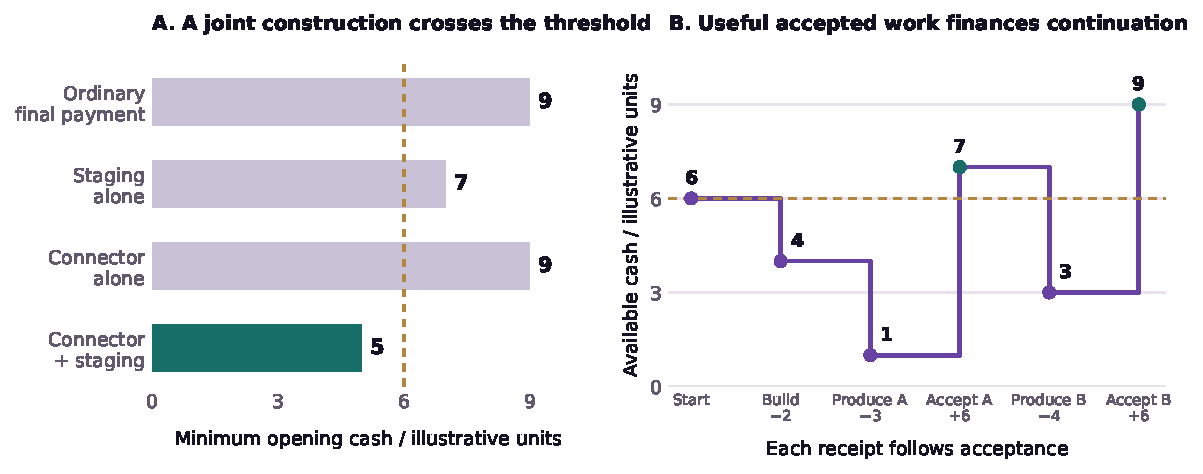
\includegraphics[width=\linewidth]{figures/construction.pdf}
\caption{Exact analytical witness. Left: the opening-capital threshold of each complete route. Right: the joint route uses receipts only after a useful stage is accepted. The dashed horizontal line is the available starting capital, not a universal capital restriction.}
\label{fig:construction}
\end{figure}

The constructive change is therefore specific. It creates a useful intermediate output early enough for voluntary earned payment to finance continuation. Staging a promise without such an output would not satisfy the model. Merely relabeling a payment would not repair the ordinary path's seven-unit initial requirement. The connector's productive effect is a supplied hypothesis in this witness, not a technology autonomously discovered by the companion.

\subsection{Additional burdens remain visible}
The nine-unit envelope is an analytical process specification, not a measured complete commercial invoice. Let $h\ge0$ represent an additional common lifecycle burden, paid before the process begins. It can stand for otherwise unmodeled discovery, acquisition, administration, financing or residual obligations. The joint route then requires $5+h$ opening units and leaves surplus $3-h$. At the fixed opening balance of $6$, it can execute only when $h\le1$; its surplus is positive only when $h<3$.

This sensitivity prevents an included computation from becoming an assertion of free economic resources. If an additional burden occurs later, its actual timing belongs in the cash plan. If the delivery can fail or incur refunds, the corresponding branch and protections must be modeled. The fixed deterministic trace establishes only its declared execution. It is not a native enterprise account and does not overwrite any laboratory financial history.

\subsection{The conventional constructor has the same freedom}
The complete conventional control can choose every supplied production route and every allowed contract. It finds the same feasible joint arrangement at opening cash $6$. The constructive result is real within the model; an inventor-superiority result does not follow.

Changing capital also changes the best choice. At $7$, ordinary staging becomes feasible and can tie the three-unit surplus without the new connector. At $9$, an ordinary final-only route can offer only the complete bundle for $13$. With value $14$, the buyer strictly prefers that purchase to refusal; the four-unit surplus exceeds the staged route's three. This pure-bundle offer does not advertise the cheaper component purchases, and it receives no early stage payment. It is a legitimate, stronger complete alternative when the initial cost can be funded.

The companion evaluates these route and price choices within a declared finite domain. No route receives hypothetical credit. A separately specified, voluntarily supplied financing contract could change the ranking, with its cost and repayment included. The calculation therefore identifies where a joint construction helps under a resource boundary; it does not establish that the selected capital is globally optimal or that the joint route is always preferable.

There is also an instructive tie in the original menu: values $7,7,14$ and posted prices $6,6,13$ give single-purchase utilities $1,1,1$. One cannot infer that a single-purchase buyer pays $13$. The cart yields utility $2$ and payment $12$. The study preserves refusal and indifference rules explicitly rather than selecting the buyer action that makes the seller's claim look best.

\subsection{A strategic omission can invent a fictitious successor}
After the executed joint route, cash is $9$. A projection that substitutes the advertised joint quote of $13$ for the actual aggregate receipts of $12$ would report cash $10$. It would therefore appear to fund a successor requiring ten upfront units, even though the actual route is one unit short. This is a deliberately authored illustration of Equation~\ref{eq:leakage}; the $13$ receipt is a naive quote-based projection, not a rational single-purchase result for this menu.

Profit and cash remain different. The first route's three-unit surplus does not mean that only three units of cash exist. A four-unit successor is affordable from the actual nine-unit balance, subject to the stated zero remaining obligations. That funding would use a mixture of opening capital and earnings unless a separate attribution establishes otherwise. Protecting the entire initial capital solely to manufacture a stronger enabling result would change the experiment.

On a subsequent use, the retained connector avoids its two-unit reconstruction cost. The fresh process costs $7$ and can leave surplus $5$ at the same twelve-unit receipts. Rebuilding costs $9$ and leaves $3$. Ordinary reuse of identical connector content ties the retained method. This is a fixed-menu, fixed-schedule inheritance comparison. The improvement is attributable to the available artifact, not to a demonstrated improvement of the invention procedure; the first construction cost remains in the two-episode history.

The stronger adaptive continuation should also be used. On a fresh task whose offer need not retain the earlier component commitments, the retained connector can support final-only production costing $7$ and a pure-bundle receipt of $13$. The first episode's closing cash of $9$ funds that path. The second surplus is then $6$, total two-episode surplus is $9$, and cash ends at $15$. An ordinary controller with the same asset and choices ties. Fixing the earlier staged contract indefinitely would miss a legitimate improvement made possible by the changed state.

\subsection{Exact verification and its domain}
The companion enumerates 2,187 three-service price menus, corresponding to seven nonempty service sets with prices in $\{1,2,3\}$. The union-graph calculation agrees with independent enumeration of 279,936 carts and all 413,343 buyer-and-budget comparisons. It also checks 139,968 subadditivity inequalities and 15,309 coordinatewise price increases, along with contractivity and idempotence. These are exhaustive finite checks, not independent market observations.

A separate two-service search considers 4,096 menus, with each price either absent or in $\{0,\ldots,14\}$. It preserves explicit best responses, budgets and non-entry. Allowing carts raises seller receipts in 341 menus, lowers them in 91 and leaves them unchanged in 3,664. The effective joint quote is lower than the posted joint quote in 560 menus. Thus the fixed-choice regret result does not imply that adding buyer options always lowers actual revenue: the selected outcome can change. Both complete pricing methods identify the pure-bundle-only price $13$ as a revenue optimum in this one-shot domain.

The separate joint price-and-route search evaluates 480 contracts plus non-entry. At opening cash $6$, 126 contracts satisfy the modeled buyer participation conditions, 28 are financeable and six have positive surplus. The best feasible arrangement uses the connector and staged prices $(6,6)$, producing surplus $3$. At opening cash $9$, ordinary pure bundling produces surplus $4$. The independent conventional control has every same choice and ties both optima. Twenty-four focused tests pass, including false equivalence, unsupported unions, exact budgets, buyer ties, financial timing, overhead and the stronger successor continuation.

These finite calculations establish exact agreement and conditional optima within their supplied domains. They are not estimates of real behavior, a statistical confirmation set, or evidence that the program invented the service primitives. The source includes the protocol, executable companion, independent cart oracle, focused regressions, deterministic result file and the plotted trace. Appendix~\ref{app:proofs} states the mathematical assumptions, and the reproduction guide explains how to regenerate the checks and paper.

\section{From a viable arrangement to a consequential successor}\label{sec:succession}
An economic game becomes part of a flywheel when what it produces changes the next useful possibility. The important inheritance can be available earnings, a qualified instrument, a reliable interface, a verified relationship, information about failure, or a procedure for constructing related instruments. Each has a different causal role.

The new example connects these roles in a deliberately small setting. A connector changes when a useful accepted output can be produced. A staged voluntary contract converts that output into an earned receipt. Actual composed purchases determine the receipt's amount. Available funds and the retained connector then change the next feasible construction. Removing any of these links changes the explanation of what happened.

\subsection{Retain an executable capability, with its limits}
A reusable mechanism can be represented as
\begin{equation}
M:(X,S,R)\longrightarrow(Y,S',E),
\end{equation}
where $X$ is the permitted input, $S$ the relevant initial state, $R$ the resource and rights contract, $Y$ the delivered output, $S'$ the resulting state, and $E$ the acceptance evidence. The representation also needs prerequisites, failure behavior, invalidation conditions and a stopping rule.

A useful composite can become a mechanism in its own right. It may hide routine internal detail while exposing the distinctions that matter to future work. This can reduce repeated reasoning and make a longer construction feasible. It can also hide a shared resource conflict, a correlated error or a new strategic action. Composition therefore requires checking both the interfaces and the coupled state: two independently valid promises can depend on the same available cash, capacity or exclusive right.

The inherited object should include what it can do, when it may fail, and how it was established. A technical certificate can remain valid after a buyer obtains a better outside option. The corresponding commercial certificate may then expire. Likewise, a useful method can transfer without carrying permission to contact a new party, spend money or operate a physical device. Acceptance, commercial applicability and authority are separate parts of reuse \cite{world,outevolve,foundation}.

\subsection{Test financing and capability as different explanations}
Suppose a first arrangement pays for a second. That establishes a funding relation only if the required funds actually become available in time and the expenses are recorded. It does not show that the first arrangement's invention was needed to produce the second output. Conversely, an inherited instrument can lower the successor's required capital without the parent's earnings paying every expense.

For a capability claim, compare the successor with and without the named asset under matched starting resources and an explicitly declared information boundary. The alternative may buy, rebuild, substitute, reorganize the work or decline. Removing the candidate's instrument while denying the control the corresponding resources is not a strong causal comparison. When the control rebuilds the same instrument economically, the result can still be useful inheritance, but not exclusive enablement.

In the analytical witness, reuse saves a two-unit construction expense. An ordinary operator given the same connector receives the same saving. This is a positive retained-capability result and a conventional tie. The first construction's expense remains in the complete history; it is not erased because later deliveries are cheaper. A succession sequence should report both incremental successor cost and total acquisition-plus-use cost.

Finance has its own matched comparison. Vary capital or financing while keeping the productive means fixed, and include the timing, fees, repayment, dilution or control terms relevant to the proposed funding. A modeled lender is another strategic participant with an outside option, not a source of free money. The initial capital choice belongs in prospective design. Historical experiments that began with US\$100,000 retain that starting condition; they do not make it a universal restriction on future arrangements \cite{superalpha}.

\subsection{Measure what becomes reachable}
For a declared capability state $K$, information $H$, resource envelope $B$ and legitimate constraints $d$, let $\mathcal R(K,H,B;d)$ denote the outcomes reachable through the supported complete routes. This is an operational set, conditioned on what can be discovered, constructed, financed and accepted within that boundary. It is not the set of everything physically possible to an omniscient planner.

A useful invention can enlarge the tested reachable set or reduce the resources required to reach a known outcome. A complete claim must identify the added outcome or changed requirement, the accepted route and the strongest feasible alternative. Unknown alternatives remain unknown. The scalar value of an uncertain future opportunity can inform planning, but does not become current revenue, capital or a demonstrated successor.

The reachable set can also contract. A formerly useful interface may become incompatible. A supplier may withdraw. A rival can reproduce a technique and improve the buyer's outside option. An obligation can consume the cash that previously appeared available. A continuing enterprise must re-evaluate the state and choose among delivery, acquisition, repair, further invention, financing and keeping cash. No fixed research fraction or compulsory novelty quota is implied.

\section{A better toolkit is not yet a better inventor}\label{sec:inventor}
The strongest recursive claim concerns the procedure that discovers and constructs arrangements. More capable starting tools can improve later performance even when that procedure is unchanged. A larger collection of examples can improve lookup without improving invention. Better ordering can reduce one search counter while remaining more expensive than direct conventional use. Each can be worth retaining, but they are different explanations.

To test improvement of the inventor, fix a fresh task distribution or a declared finite task set, the relevant acceptance condition, rights and complete resource accounting. Compare an earlier construction procedure $L_0$ with a retained successor procedure $L_1$ while controlling the initial tools and information. Let $J(L,K)$ be accepted task value net of the declared complete burden, with larger values preferred. Then
\begin{equation}
\Delta_L(K)=J(L_1,K)-J(L_0,K)
\end{equation}
measures a procedure difference at fixed starting capability. Crossing old and new procedures with old and new capabilities separates that effect from equipment and their interaction \cite{outaccelerate,superalpha}. A further equal-content ordinary-reuse control tests whether the benefit comes from an improved constructor or simply having the same useful material available.

\begin{table}[ht]
\small\centering
\begin{tabularx}{\linewidth}{@{}P{3.2cm}YY@{}}\toprule
Claim & Decisive comparison & Common confound\\\midrule
Useful composition & Complete constructed arrangement versus capable separate and integrated routes & Giving only the candidate the missing interface\\
Capability inheritance & Fresh successor with the retained asset versus equally resourced purchase, reconstruction or substitution & Free acquisition or a deliberately disabled control\\
Improved discovery & Changed procedure versus old procedure and strong conventional construction with equal starting content & A better toolkit mistaken for a better searcher\\
Improved commercial result & Complete policy under credible participant and rival responses, including non-entry & Assumed demand, missing expenses or uncollected invoices\\
Physical expansion & Qualified installed capability and useful throughput under real resource constraints & Revenue or a simulation counted as a working facility\\\bottomrule
\end{tabularx}
\caption{The comparisons address different claims. An arrangement can succeed commercially without demonstrating every form of recursive improvement.}
\label{tab:claims}
\end{table}

\subsection{Count the cost of becoming better}
The acquisition of a procedure consumes resources even if its later use is cheap. Include unsuccessful candidates, checking, integration, maintenance and the cost of obtaining reusable evidence. If costs are amortized over a reuse horizon, declare that horizon and distinguish completed reuse from hoped-for future demand. A measured number of solver calls or constraint rows is not automatically a monetary cost. Unknown actual billing remains unknown.

The primary AI-versus-human productivity comparison should use competent frontier AI or agents against competent human workers using conventional software, with the same complete outcome, quality, rights and obligations. Other autonomous providers, human-plus-AI providers, self-service and non-purchase are separate commercially relevant alternatives. An authored simulator is not a measurement of either labor arm. Actual human intervention inside an otherwise autonomous operation must be counted; ordinary buyer consent is participation, with its own friction, rather than invented internal human labor.

\subsection{Let the stronger method remain the incumbent}
The invention engine should be permitted to simplify itself. If an unrestricted conventional optimizer finds the same arrangement with less total burden, operating that optimizer is a sensible outcome. A complex critic-and-builder loop is not an end in itself. Useful retained counterexamples may improve reliability even when their original search procedure is retired.

This principle also governs stopping. A finite campaign should declare its candidate domain, work budget, comparison arms, acceptance conditions and stopping rule before its confirmation results are used. Stop when the registered task is completed, the budget is exhausted or the intended claim is falsified; preserve the outcome. A subsequent broader search can be justified and registered separately. Repeatedly changing the evaluator or restarting exposed cases until something wins does not establish improvement.

The current exact companion is an exhaustive authored calculation, not an untouched statistical holdout. Its finite enumeration terminates after the stated domain is evaluated. The open research objective is to discover useful new productive representations and arrangements beyond such supplied domains, then demonstrate a fresh advantage after complete costs.

\section{What the current machinery establishes}\label{sec:evidence}
The conceptual program is accompanied by a growing finite engineering substrate. The relevant public work is Omega PR~201, reviewed here at commit \nolinkurl{8cd375784c24b879ae1eb4835c6af4fb925cbf4c}. At the review snapshot the pull request is open, draft and unmerged. The V3 report and evidence were committed at \nolinkurl{870a4e8822c89583ca89b7cad729cb830237da53}; the later V4 protocol records the compositional counterexample \cite{omegav3,omegav4}. These identities define the evidence used here, irrespective of subsequent branch development.

\subsection{A working finite construction and operating loop}
V3 automatically constructs deterministic allocation and payment programs from an authored public market specification. The constructor receives the prior type distribution, permitted outcomes, costs and budgets, not the particular buyer's realized private valuation. Ordinary mixed-integer optimization proposes the program. An independent integer verifier checks the supported unilateral reports, participation, budgets and outside options.

Rejected candidates can supply additional incentive constraints. Retained constraint structure is reused as a search hint; every new program still faces the complete supported verifier. The operating path then executes existing source-grounded KPI and reconciliation work, checks its outputs and settles simulated payments through the existing \texttt{JournalAccount}. It does not create a parallel ledger. Positive runs fund a checked successor from available earnings.

This is an achieved finite engineering loop: construction, criticism, correction, checking, useful execution, modeled settlement and continuation. Its primitive services and market language are supplied. Its incentive boundary is the historical single-purchase game. The independently replayed cart counterexample identifies a further condition required before extending that claim to composed purchases.

\subsection{Strong controls change the scientific verdict}
Three nine-type V3 markets compare the generated mechanism with the best separate-or-bundle offer and an unrestricted conventional optimizer within the same finite mechanism class. All receive the same modeled outcomes, costs, budgets and participation conditions.

\begin{table}[ht]
\small\centering
\begin{tabularx}{\linewidth}{@{}Yrrr@{}}\toprule
Market & Generated & Best standard & Full conventional\\\midrule
Complementary & $55013/37$ & $55013/37$ & $55013/37$\\
Substitute & $22503/29$ & $22503/29$ & $22503/29$\\
Competitive & $6001/8$ & $29377/40$ & $6001/8$\\\bottomrule
\end{tabularx}
\caption{Historical V3 expected contribution in cents under its single-purchase model. Fractions are exact. These are authored type-weighted expectations, not observed market averages.}
\label{tab:v3mechanisms}
\end{table}

The competitive case gains 15.7 cents, about 2.14\%, over the best standard-offer arm in that original model. The full conventional optimizer ties in every market. The cart obstruction prevents promoting the competitive result to an advantage robust to composed purchases. It does not erase the exact original comparison or establish that its arithmetic was wrong.

The retained search builds 1,140 constraint rows, compared with 1,253 for the same procedure started cold: 113 fewer, or about 9.02\%. The full conventional optimizer needs 999 rows and has lower observed construction CPU in the reported run. The retained method therefore improves one matched predecessor comparison without establishing that it is the strongest operating method. Constraint counts and CPU are telemetry, not inferred monetary savings.

An earlier V2 study makes the distinction equally visible. Automatically inherited search order reduces mapping work from 265,020 to 227,614 units, approximately 14.1\%. Yet acquiring and using the retained procedures costs 238,126 measured units, versus 75,456 for direct predecessor use; a fixed conventional method matches output quality with 10,512 use units, with its historical development cost unmeasured \cite{omegav2}. An improvement relative to one's own search baseline is not a complete-lifecycle advantage over the strongest feasible alternative.

\subsection{Native accounts retain their original meaning}
V3 reports five distinct native simulated businesses. Each begins with its own US\$100,000 and executes a sparse 365-day authored schedule with one opportunity for each of 27 synthetic types. These opportunities are not an empirical demand sample or a draw from the expectation weights in Table~\ref{tab:v3mechanisms}.

\begin{table}[ht]
\small\centering
\begin{tabularx}{\linewidth}{@{}Yrrr@{}}\toprule
Historical arm & Collections & Expenses & Modeled profit\\\midrule
Generated mechanism & 265.400 & 132.824 & 132.576\\
Best standard offers & 257.170 & 129.618 & 127.552\\
Full conventional mechanism & 265.400 & 132.824 & 132.576\\
Generated, copycat outside option & 0.000 & 49.700 & $-49.700$\\
Generated, no demand & 0.000 & 49.700 & $-49.700$\\\bottomrule
\end{tabularx}
\caption{Separate historical V3 simulations, in US dollars, under authored tariffs and the original single-purchase semantics. No accounts are pooled, reinterpreted as cart-corrected operations, or annualized.}
\label{tab:v3finance}
\end{table}

The generated and full conventional arms each serve 20 paying buyers; the standard arm serves 19. The generated advantage over standard is US\$5.024 of modeled profit, approximately 3.94\%, and the full conventional arm ties. Both adverse arms incur a loss. A copied offer is one feasible outside-option stress, not a claim to have solved a rival's globally optimal strategy.

Each positive arm includes a US\$5 expense for a successor mechanism, paid from unrestricted earnings after the declared maintenance and tax provision. The successor executes and passes the finite incentive verifier. This is evidence of earned funding and successful execution. It does not establish that an equally funded ordinary route could not have constructed the successor.

The historical evidence records source-matched financial and operating audits and a completed-account resume that leaves the financial export unchanged. It also records 25 semantic and learning tests plus eight native fault tests in two completed invocations. Those records are not a claim that this paper reran every account, that all present-main dependencies were requalified, or that the branch became a released production system.

\subsection{Complete modeled expenses and actual economic costs}
The native audit reconstructs the declared setup, discovery, acquisition, delivery, checking and support, collection fees, maintenance, tax and successor charges. The tariffs are authored resource envelopes. Actual model, developer and host lifecycle costs remain unknown; included execution does not establish a zero economic cost. Actual customer revenue in these studies is zero.

These limits are consequential. The record supports scoped automatic mechanism construction and audited conditional commerce. It does not establish empirical demand, durable competitive advantage, general productive invention, a better open-world inventor, or the laboratory's US\$3 billion trailing-365-day complete-cost profit objective. The purpose of the paper is to turn the observed boundary into a sharper constructive objective and a reproducible test, while preserving what the system has already achieved.

\section{The larger opportunity}\label{sec:horizon}
The motivating consequence is much larger than a better tariff. Many useful activities need several missing conditions to become an industry: a way to produce the result, a way to recognize it, a workable division of effort, a financing path and enough voluntary demand. Intelligence applied to that whole construction could make previously impractical cooperation repeatable.

The first consequential prototype should test a missing condition that matters beyond one convenient example. A small, decisive experiment can establish a large enabling relationship. Its ambition comes from the class of useful work it could open, not the size of a speculative market total or the number of agents assigned to it.

\subsection{Scientific capability as a shared productive service}
Suppose several research users need measurements that are individually too expensive to obtain. A construction might combine a reusable instrument, calibrated evidence and agreements that allocate access and support. The technical task is to obtain the required information reliably. The economic task is to make contributions, capacity and risk worthwhile for each participant. The strategic task includes alternative measurements, shared purchases, data derivation and competing suppliers.

The decisive first test would deliver a specific useful measurement under an independent acceptance condition, compare the strongest complete alternative, and then use the retained instrument on a distinct investigation. If the second investigation can already be done more cheaply with available equipment, the claimed enabling residual disappears. If it benefits only because the same data were handed to it, that is a content-reuse result. A stronger successor claim needs a new useful investigation and an attributable construction benefit.

\subsection{Industrial cooperation made possible by evidence}
Independent operators may possess complementary capacity while lacking a dependable way to coordinate its use. A productive arrangement could construct the required measurement, control interface and acceptance method, then allocate work and exposure under voluntary terms. A qualified intermediate output can permit earned progress payments; a meaningful measurement can make a contingent commitment credible.

The first test should measure the actual industrial outcome: conforming throughput, useful energy, reliable availability or another explicit beneficiary target. Settlement, maintenance, interruptions, shared resources and adverse conditions belong in the same arrangement. A simulated schedule does not operate equipment. A profitable model does not establish physical capacity. Moving to real devices requires the relevant engineering evidence and operating authority \cite{frontier}.

\subsection{A foundry for complete useful arrangements}
A broader foundry could construct and adapt the interfaces, verification routines and operating methods that connect specialist capabilities. The commercial product would be a useful accepted outcome or an independently usable productive capability. A simple existing tool may supply most of the answer; the valuable invention may be the small connector that removes a consequential obstacle.

Such a foundry should also search for ways to eliminate a dependency. If an inherited workflow requires reconstructing an unavailable state, the useful intervention may be a decision rule that needs less information. If repeated verification is expensive, a qualified production interface may make the relevant property directly checkable. Constructing every missing component of the original workflow is not always the best route to the authorized purpose \cite{ti,world,original}.

Each successful composite can become a candidate operator for further construction, with explicit applicability and invalidation conditions. A constructor of useful composites can itself become a retained object. This is the recursive ambition: the enterprise becomes better equipped to invent the conditions of subsequent progress. That last improvement must still earn the comparisons in Section~\ref{sec:inventor}.

\subsection{Create enough value to sustain the creator}
The enterprise needs a defensible share of the value it helps produce. Possible sources include superior accepted outcomes, reliable integration, calibrated evidence, shorter qualification, useful service continuity, scarce complementary assets and continuing productive invention. The relevant source depends on the market. A freely available implementation can make adoption and independent use easier, while a service or complementary productive asset remains costly to reproduce. None of those possibilities establishes willingness to pay on its own.

The created capability can also lower a rival's cost or let a buyer self-produce. This can be socially valuable while weakening the creator's margin. An invention program must therefore evaluate participant and competitive response alongside production. It should pursue a new instrument, a better delivery process, a new customer opportunity or retaining liquidity according to their evidence and complete consequences. Sustaining the enterprise is a real design problem; manufacturing dependence is not a substitute for creating value.

The laboratory's US\$3 billion objective concerns profit over a complete trailing 365-day window after modeled costs. It remains unachieved in the evidence reviewed here. Capital, financing, demand, price, repeat business, capacity, risk and competitive response all affect whether such a scale can be reached. There is no universal game-theoretic optimum without specifying those conditions, the feasible strategies and the objective. A finite optimum in the companion certifies only its supplied domain.

\section{A concrete engineering objective}\label{sec:objective}
An achieved autonomous economic-game inventor should be describable in operational terms. Given an authorized purpose and a declared environment, it constructs an executable arrangement, obtains the evidence needed to evaluate it, exposes consequential strategic and productive defects, and repairs or rejects the candidate. When a candidate is selected, it funds the required actions, delivers accepted work, settles the modeled or actual payments and carries the complete obligations. It retains useful means and tests their contribution to fresh successor work.

This objective has a meaningful bounded version. A system can complete that loop within an explicit finite language and environment. Its achievement should be reported with that boundary, including which primitive capabilities, type distributions, valuations, cost models and construction procedures were supplied. The broader version additionally requires discovery of materially new means or arrangements, robust advantage against capable alternatives, and evidence that retained procedures improve future invention after their acquisition cost.

For a consequential next experiment, select a beneficiary outcome with a clear missing condition and compare materially different routes: direct production or purchase, a new productive construction, and a different arrangement of evidence, commitments or work. Give the strongest complete alternative the same relevant freedom. Freeze the accepted outcome and finite comparison. Construct the smallest useful instrument that could decide the issue, then execute an entire funded episode if the evidence supports it. A failed test can identify the next construction or justify non-entry; it should not disappear from the cost history.

The publication and its companion support that work by clarifying one connection that a correct optimizer can miss: a productive invention changes the economic actions available to participants, and those actions change the resources available to the successor. The current finite engineering record already contains functioning mechanism construction, checked service production, simulated settlement and earned-funded continuation. It also contains conventional ties, adverse losses and a specific omitted-action failure. Those facts make the next construction more concrete.

\thesis{A lasting flywheel creates a possibility that works, leaves useful means behind, and earns the ability to construct what comes next.}

The research program is therefore both ambitious and falsifiable. Its unit of progress is a consequential accepted arrangement and a demonstrated successor relation. Its long horizon is an expanding repertoire of useful scientific, industrial and organizational capabilities. The work ahead is to make the machine increasingly able to discover and construct those arrangements, while participants remain free to choose and the evidence remains strong enough to tell us when it has succeeded.

\appendix
\section{Formal assumptions and proofs}\label{app:proofs}

The results below are elementary deductions for declared finite models. They connect known ideas in arbitrage-free pricing, mechanism design and program synthesis to the paper's constructive question \cite{datapr,conitzer2002,synthesis,cegis}. Their proofs establish those conditional statements; they do not establish empirical demand, unrestricted incentive compatibility or an autonomous invention advantage.

\subsection{Composition and the effective price}\label{app:closure}

Let $G$ be a finite set of services. A posted menu $\mathcal M\subseteq 2^G$ contains $\varnothing$ at price zero and assigns a finite nonnegative price to each offer. Let
\[
\mathcal F=\left\{\bigcup_{B\in\mathcal B}B:\mathcal B\subseteq\mathcal M\right\}
\]
be the complete family of reachable unions. Thus $\mathcal F$ is finite, contains $\varnothing$, and is closed under union. Extend $p$ to $\mathcal F$ by assigning $+\infty$ to outcomes not individually posted. Every member of $\mathcal F$ still has a finite-price implementing cart.

The model requires more than a set representation. Every modeled combination must be permitted and executable. A cart delivers its union exactly once; repeated purchases add no service. The accepted output, quality, timing, rights, warranty and other material effects are the same for all carts with the same union. Payment is the sum of offer prices, with no omitted cart fee or composition cost. There are no conflicting capacity or permission constraints. These are assumptions to verify against the actual productive system, not consequences of the notation. Under them, removing repeated offers never increases cost, so a minimum over finitely many carts exists.

Define the effective tariff by
\begin{equation}
(\mathsf Cp)(S)=
\min_{\substack{\mathcal B\subseteq\mathcal M\\\cup_{B\in\mathcal B}B=S}}
\ \sum_{B\in\mathcal B}p(B),\qquad S\in\mathcal F.
\label{eq:appendix-closure}
\end{equation}
The empty cart has union $\varnothing$ and price zero. A tariff $q$ is \emph{union-subadditive} when $q(A\cup B)\le q(A)+q(B)$ for every $A,B\in\mathcal F$.

\begin{proposition}[Effective tariff and budget-preserving equivalence]
\label{prop:closure}
On the fixed domain above, $\mathsf Cp\le p$, the operator $\mathsf C$ is monotone under pointwise price order, and $\mathsf C(\mathsf Cp)=\mathsf Cp$. Moreover, $\mathsf Cp$ is the greatest nonnegative union-subadditive tariff $q$ with $q(\varnothing)=0$ and $q\le p$.

For a buyer with quasilinear utility $v(S)-x$, $v(\varnothing)=0$, hard budget $b\ge0$, and a zero-utility decline option, the maximum utility from feasible carts is exactly
\begin{equation}
\max\left\{0,\ \max_{\substack{S\in\mathcal F\\(\mathsf Cp)(S)\le b}}
\bigl[v(S)-(\mathsf Cp)(S)\bigr]\right\}.
\label{eq:appendix-buyer}
\end{equation}
The maximizing delivered-outcome/payment pairs agree between the cart model and this effective-tariff model.
\end{proposition}

\begin{proof}
Every individually posted offer is a feasible one-item cart, so $\mathsf Cp\le p$; the inequality at unposted outcomes is immediate. If $p\le p'$ on a common reachable domain, every finite cart under $p'$ is available under $p$ at no larger cost. Minimizing gives $\mathsf Cp\le\mathsf Cp'$.

The union of minimizing carts for $A$ and $B$ implements $A\cup B$ at cost no larger than their sum, after removing any repetitions. Hence $\mathsf Cp$ is union-subadditive. If $q\le p$ is any other union-subadditive tariff, repeated application of its inequality gives
\[
q(S)\le\sum_{B\in\mathcal B}q(B)
       \le\sum_{B\in\mathcal B}p(B)
\]
for every cart implementing $S$. Taking the minimum yields $q\le\mathsf Cp$, proving greatestness. Applying this property to the already subadditive tariff $\mathsf Cp$ proves idempotence.

Finally, any affordable cart delivering $S$ costs at least $(\mathsf Cp)(S)$. Replacing it by a minimizing cart preserves affordability and weakly improves utility, strictly so when its price falls. Conversely, the defining minimum supplies an affordable implementing cart for every outcome admitted in \eqref{eq:appendix-buyer}. This proves the equality and the correspondence of optimal outcome/payment pairs, including decline.
\end{proof}

The result preserves the full best-response correspondence. A selected revenue still requires a common tie convention, or a reported range over ties. A buyer's maximum utility alone does not determine seller revenue when several different outcomes attain it. The finite study makes refusal and seller-unfavorable ties explicit.

One implementation uses a graph with nodes $U\in\mathcal F$ and edges
$U\to U\cup B$ of weight $p(B)$ for each posted $B$. Set $D(\varnothing)=0$ and minimize the path weight to every reachable union. Nonnegative self-loops can be discarded; every remaining edge strictly enlarges the service set. Relaxing edges in increasing set cardinality therefore computes $D(S)=(\mathsf Cp)(S)$ in $O(|\mathcal F|\,|\mathcal M|)$ arithmetic operations. Enumerating all subsets of posted offers supplies an independent small-case control. The state space can itself be exponential in $|G|$; this is not a general efficient algorithm for unrestricted productive composition.

If combining services changes quality, rights, production costs, settlement timing or permissible use, those distinctions belong in the state and acceptance contract. The set-union reduction then requires revision. It does not cover resale, coalitions, multiple identities, repeated consumption, strategic default, intertemporal commitments or general query determinacy. Query-based data pricing studies a richer information-determinacy relation \cite{datapr}.

\subsection{What expanding the strategy model can invalidate}\label{app:strategy-expansion}

For a fixed mechanism $m$, buyer type $\theta$ and intended action $a^*$, let $\mathcal D\subseteq\mathcal D'$ be two sets of feasible actions, both containing $a^*$. Utility for every action in $\mathcal D$ must remain the same in the two models. Define
\[
\operatorname{Reg}_{\mathcal D}(m,\theta,a^*)
 =\max_{a\in\mathcal D}\{u(m,\theta,a)-u(m,\theta,a^*)\}.
\]

\begin{proposition}[Fixed-payoff strategy expansion]\label{prop:regret}
For the nested action sets above,
$\operatorname{Reg}_{\mathcal D'}\ge\operatorname{Reg}_{\mathcal D}$.
Consequently, among a fixed set of candidate mechanisms with unchanged payoffs, the candidates with regret at most $\varepsilon$ for every tested participant/type under $\mathcal D'$ form a subset of those passing under $\mathcal D$. An analogous set inclusion holds for a fixed-profit function's worst-case lower bound over nested response sets.
\end{proposition}

\begin{proof}
Maximization over a superset cannot decrease a maximum. Apply that inequality to every required participant/type constraint. For the last statement, an infimum over a larger response set cannot increase.
\end{proof}

This does not imply that actual equilibrium revenue always falls when actions are added. It also does not say that better productive means cannot help: a new construction can change costs, payoffs and the candidate arrangements themselves. The proposition applies to the narrower question of whether an existing certificate survives a more complete strategy model with its common payoffs held fixed.

\subsection{A collection error can cross a funding boundary}\label{app:leakage}

\begin{proposition}[Conditional successor funding gap]\label{prop:leakage}
Fix one intended, accepted sale of $S$ in a deterministic cash sequence. Let $u$ be unrestricted cash before its production outlay, $c$ the cash outlay attributable to that sale, $r\ge0$ the additional amount that must remain protected afterward, and $K\ge0$ the upfront successor commitment. Suppose all earlier events are feasible, there are no other intervening flows, the buyer actually chooses $S$, and composition changes only the collected price, from $p(S)$ to $(\mathsf Cp)(S)$.

The advertised-price calculation permits that commitment while the actual collection does not exactly when
\begin{equation}
u+(\mathsf Cp)(S)-c-r<K\le u+p(S)-c-r.
\label{eq:appendix-leakage}
\end{equation}
The actual additional cash required is
$K-[u+(\mathsf Cp)(S)-c-r]$, which is positive and no larger than $p(S)-(\mathsf Cp)(S)$.
\end{proposition}

\begin{proof}
The two post-sale available balances differ by precisely
$p(S)-(\mathsf Cp)(S)$. Affordability means that the relevant available balance is at least $K$; applying that test to both balances gives \eqref{eq:appendix-leakage} and the stated shortfall bound.
\end{proof}

The restriction to the same realized output is material. A changed effective tariff can also change the buyer's chosen outcome, participation, production cost and timing; those cases require re-solving the full route. The protected amount $r$ must arise from an actual declared obligation or reserve rule. It cannot be invented afterward to make a desired funding result hold. Profit, cash and the attribution of financing to earned receipts remain separate, as in the predecessor's ordered-cash analysis \cite{superalpha}.

\subsection{The staged construction and its participation conditions}\label{app:staging}

The authored two-service construction keeps the complete reference expense at nine units while changing when useful accepted work can be delivered. Ordinary final-only delivery costs nine upfront. Ordinary staging costs seven before accepted $A$ and two afterward. The connector costs two to build and permits accepted $A$ at cost three, followed by $B$ at cost four. Connector construction plus final-only payment still requires nine upfront. Both component prices are six; the posted joint price thirteen is dominated by the twelve-unit cart.

At opening cash six, the joint connector-and-staging path is
\[
6\xrightarrow{\text{construct }2}4
 \xrightarrow{A\text{ costs }3}1
 \xrightarrow{A\text{ pays }6}7
 \xrightarrow{B\text{ costs }4}3
 \xrightarrow{B\text{ pays }6}9.
\]
The four minimum capital requirements are respectively $9,7,9,5$. For example, ordinary staging needs at least seven for its first output; after its six-unit receipt, capital seven leaves six, which covers continuation cost two. The joint route needs five for construction and the first output; that first receipt then covers continuation cost four. These ordered balances prove necessity and sufficiency under the fixed path assumptions. The same total expense nine and receipt twelve produce profit three whenever a route is executable.

This four-route comparison fixes component prices and accepted deliveries to isolate the liquidity effect. It is not a price-optimality claim. With integer prices and refusal at zero surplus, an independently voluntary purchase of either seven-unit component can charge at most six. A different menu containing only the joint offer at thirteen is accepted for value fourteen and yields profit four, but requires nine upfront under the declared final-only route. At opening seven ordinary staging can tie the joint construction; at opening nine pure bundling can exceed its profit. The quoted joint price thirteen in the menu $(6,6,13)$ must also not be confused with guaranteed revenue in a restricted single-purchase game: all three individual offers then give utility one, and seller-unfavorable ties can select a component. The composed cart gives utility two and strictly wins.

Each payment is earned only after independent acceptance of a useful output. The assumed buyer values are $v(A)=v(B)=7$ and $v(A\cup B)=14$, with sufficient cash to pay each six-unit installment. No better external offer is present in this particular authored instance. Accepted $A$ remains useful if continuation is declined, so its one-unit standalone surplus does not depend on a later promise. Given $A$, accepted $B$ adds value seven at price six. The continuation choice is therefore strictly worthwhile. Both parties can perform and settle the declared accepted exchange; enforcement and payment certainty are assumptions, not findings about an actual buyer. The composition model gives the same complete delivered services for twelve, with buyer surplus two.

These conditions are essential to the construction. An intermediate artifact that has no independently accepted value does not justify the first earned receipt. A refundable advance is not substituted for that receipt. Uncertain acceptance, collection or continuation requires a contingent policy with its own failure costs and liquidity constraints.

To expose an additional common lifecycle burden, charge a declared $h\ge0$ as an upfront expense in every first-episode plan. The four minimum capital requirements become $9+h,7+h,9+h,5+h$ and their completed profit becomes $3-h$. At opening six, the joint route is executable exactly when $h\le1$. This is a sensitivity statement about that payment timing. An actual unmeasured expense is unknown; $h=0$ in the reference calculation does not establish costless real research, computing or maintenance.

For a second accepted task with the same staged prices and payment schedule, retaining the connector removes its two-unit reconstruction expense: the declared incremental expense is seven and profit five. Rebuilding costs nine and earns three. Ordinary reuse of the identical connector also costs seven and earns five. The first-cycle construction cost remains in every full-history account; it is not erased when reporting the incremental successor benefit. This is a fixed-menu inheritance comparison, not an optimal two-episode policy.

The changed cash state permits a stronger continuation. With nine units available after the first episode and the connector already constructed, final-only production costs seven before collection. A fresh pure-bundle-only offer at thirteen gives the buyer positive surplus and produces the cash path $9\to6\to2\to15$. Its second-episode profit is six; total two-episode profit is nine. An ordinary controller with the same asset and contract options can make the same change. This alternative assumes that earlier component offers need not remain available for the fresh task; any continuing contractual commitment would have to be preserved. More opening capital, a legitimate credit contract, a stronger outside offer or another productive route can change the comparison further.

\subsection{What finite counterexample-guided synthesis guarantees}\label{app:cegis}

Counterexample-guided inductive synthesis is an established construction method \cite{cegis}. The following finite guarantee applies only when a verifier's counterexamples are sound constraints on every admissible solution, rather than arbitrary rejections of a current favorite.

\begin{proposition}[Finite refinement with complete verification]\label{prop:cegis}
Let $\mathcal C$ be a fixed finite family of $N$ exact specification constraints on a fixed candidate class. Start with a subset $\mathcal C_0$. At each iteration, a terminating complete solver either finds a candidate satisfying the accumulated constraints or correctly reports that none exists. A terminating complete verifier either accepts that candidate against every constraint in $\mathcal C$, or returns a violated member of $\mathcal C$. Retain each returned constraint permanently.

There are at most $N-|\mathcal C_0|$ rejected candidates, followed by at most one accepting or infeasibility solver call. An accepted candidate satisfies all of $\mathcal C$; a correct infeasibility result certifies no solution in the declared candidate class.
\end{proposition}

\begin{proof}
A candidate satisfies every accumulated constraint. Therefore a returned violated constraint is new. Each rejection strictly increases the accumulated subset of the finite family $\mathcal C$. After at most $N-|\mathcal C_0|$ such increases no further rejection is possible. Acceptance is sound by the complete verifier. If a subset of the required constraints has no solution, the full family has no solution either.
\end{proof}

The proposition does not bound useful wall-clock time, establish the truth of the specification, or guarantee numerical solver completeness. Floating-point tolerances, time limits and unmodeled strategies require separate treatment. If a productive construction adds new feasible actions, the old fixed family $\mathcal C$ may cease to describe the game. Retained constraints can be useful search hints only when their applicability is established; every resulting mechanism still faces current acceptance. Automated synthesis and dynamic mechanism design provide related, explicitly bounded formulations \cite{synthesis,dynamic}.

A second elementary bound applies to a finite candidate class even when the specification is presented differently. If a complete terminating verifier rejects only invalid candidates, every rejection permanently excludes the current candidate without excluding valid ones, and the search never repeats an excluded candidate, at most the class's cardinality of candidates can be examined. The result is a verified candidate or exhaustion of that class. Neither version certifies that the class contains the useful construction the beneficiary needs.

\section{Separating funding, inheritance and an improved inventor}\label{app:identification}

A fresh successor comparison should distinguish four starting conditions: baseline cash with no inherited artifact, baseline cash with the artifact, additional unrestricted cash with no artifact, and both additional cash and the artifact. Preserve other obligations, information, rights, prices and deadlines. Charge artifact construction or acquisition where it occurs and retain predecessor expense in the full history. Equalize what the comparator may reconstruct, buy, coordinate or finance; otherwise an apparent enabling effect may be unequal permissions or an excluded conventional route.

Within each condition, the current and proposed invention procedures receive identical available content and complete resource budgets. Compare accepted outcomes after search, unsuccessful attempts, verification, implementation and operating costs. Fresh tasks must be selected without consulting their outcomes, and declined or unfinished cases remain in the denominator. Record procedure effect at fixed resources, resource effect at fixed procedure, and any interaction separately. Ordinary content-identical reuse is required to distinguish useful memory from a better discovery procedure \cite{superalpha,outevolve,outaccelerate}.

This protocol does not require every profitable business to prove a new discovery algorithm. It is required for the stronger claim that the inventor itself has improved. The authored study demonstrates conditional constructions and comparisons; the protocol defines a further empirical burden.

\clearpage
\bibliographystyle{plainnat}\bibliography{references}
\end{document}
